\documentclass[a4]{scrartcl}

% \usepackage[ngerman]{babel}
\usepackage[utf8]{inputenc}
\usepackage{mathtools}
\usepackage{amsmath}
\usepackage{amssymb}
\usepackage{geometry}
\usepackage{scrlayer-scrpage}
\usepackage{float}
\pagestyle{scrheadings}
\clearscrheadfoot

\usepackage[backend=biber, maxbibnames=99]{biblatex}
\addbibresource{references.bib}

\setlength{\parindent}{0cm}


\geometry{
  paper=a4paper, % Change to letterpaper for US letter
  top=2cm, % Top margin
  bottom=1.5cm, % Bottom margin
  left=2cm, % Left margin
  right=3cm, % Right margin
}

\ohead{\\
Pina Kolling\\
piko0011}

\begin{document}

\section*{Summary: Lecture 2}

Summary for the chapters \textit{7.1 Complexity classes} and \textit{7.2 Hierarchy problem}. \cite{book}


\section*{Complexity classes}

\subsection*{Background knowledge:}

A complexity class is a set which contains problems with similar complexities. The complexities are examined in regards of a specific ressource, for example time or space. For the problems the most efficient solution/algorithm is analysed.

\begin{figure}[H]
\begin{center}
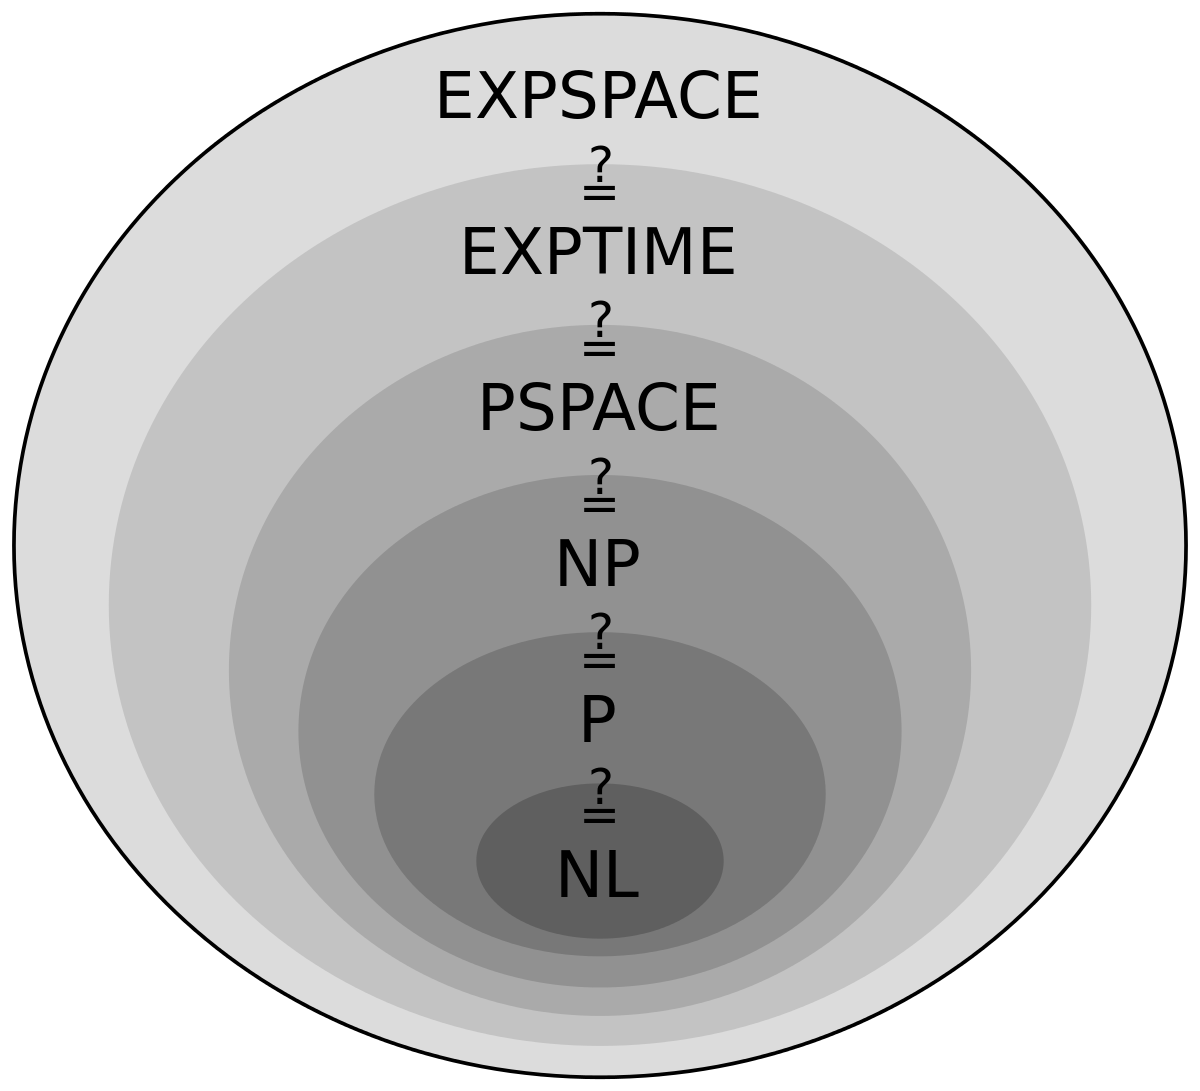
\includegraphics[scale=0.15]{images/classes.png}
\end{center}
\caption{Complexity classes \cite{classesPic}}
\end{figure}

Usually the complexity depends on the input size. With the asymptotic complexity, classes are build, which are the complexity classes. \cite{GTI}


\subsection*{Summary:}

\textbf{Parameters of complexity classes:}

\begin{itemize}
\item \textbf{Model of computation:} \\
here: multistring Turing Machine
\item \textbf{Mode of computation:} \\
for example: deterministic or non-deterministic (deterministic: the computer will always produce the same output for a given input while going through the same states, non-deterministic: can show different behaviors for the same input)
\item \textbf{Ressources:} \\ 
something \textit{expensive} that the machine uses up, for example: time or space
\item \textbf{Restrictions/Bound:} \\ 
for example: upper bound, lower bound as a function $f: \mathbb{N} \rightarrow \mathbb{N}$
\end{itemize}













%------------------------------------------------------------------




\section*{Hierarchy problem}



\newpage

\printbibliography




\end{document}